\subsection{Modélisation et identification du comportement du moteur de la Robucar}

Afin de déterminer la fonction de transfert de l'ensemble du système mécanique (moto réducteur et arbre de la roue), nous avons isolé la partie mécanique du système et réalisé un essai indiciel en introduisant un couple moteur $C_m(t)$ d'un échelon de $4N.m$ à l'entrée de l'arbre du moteur. Nous avons enregistré en sortie de la roue la variation de la vitesse angulaire comme expliqué par le schéma de la figure \ref{essai_exp}. La réponse à cette échelon est donnée figure \ref{reponse_echelon}.

On assimile la fonction de transfert à un élément du premier ordre et on relève la vitesse en régime permanent : $\Delta \dot{\theta}(\infty)=3\;rad/s$, et ceci pour un échelon d'entrée d'amplitude $C_m=4N\cdot m$.

\question{Procéder à une identification classique graphique des valeurs numériques avec les unités des paramètres caractéristiques de la fonction de transfert du 1\up{er} ordre.}


On souhaite maintenant mettre en place une méthode d'identification plus précise se basant sur la \textbf{méthode des moindres carrés}.
Dans un premier temps, on suppose que le gain statique est identifié à l'aide de la méthode précédente.
L'ensemble des données de l'essai permettant de tracer la courbe de la figure \ref{reponse_echelon} sont stockées dans le fichier 'premier$\_$ordre.csv'

\question{Écrire le programme permettant de lire le fichier 'premier$\_$ordre.csv' et de stocker sous la forme de deux tableaux $t=\left[t_1,t_2\cdots,t_n\right]$ et $V=\left[V_1,V_2\cdots,V_n\right]$ respectivement le temps et la vitesse angulaire à chaque instant.}

\question{Tracer en fonction du temps la grandeur $ln\left(\frac{\Delta \dot{\theta}(\infty)-V}{\Delta \dot{\theta}(\infty)}\right)$. Que remarquez-vous ?}

Pour la suite on note $Y$ le tableau correspondant au calcul de : 

\begin{align*}
Y=ln\left(\frac{\Delta \dot{\theta}(\infty)-V}{\Delta \dot{\theta}(\infty)}\right).
\end{align*}

\begin{prop}[Méthode des moindres carré pour une interpolation linéaire]
On travaille ici sur un nuage de points expérimentaux donnant le vecteur $Y=\left[Y_1,Y_2,\cdots, Y_n\right]$ en fonction du vecteur $t=\left[t_1,t_2\cdots,t_n\right]$.
Cette méthode permet d'identifier une fonction linéaire approchant au mieux (au sens des moindres carrés) un nuage de points issu de données expérimentales.
Dans notre cas, la fonction linéaire recherchée est donnée par :

\begin{align*}
Y=f(t)=\alpha\times t
\end{align*}
On note $E(\alpha)$ la somme des distances au carré verticale entre chaque point de coordonnées $(t,iY_i)$ et la courbe théorique issue d'un modèle (ici $Y=\alpha\times t$).

Dans notre cas :

\begin{align*}
E(\alpha)=\sum^n_{i=1}\left(Y_i-\alpha\times t_i\right)^2
\end{align*}

La valeur de $\alpha$ qui permet de trouver la droite qui approche au mieux l'ensemble des points expérimentaux au sens des moindres carrés est celle qui minimise la grandeur $E(\alpha)$ : 

\begin{align*}
\begin{array}{ccc}
\alpha & \mbox{tel que} & \frac{\partial E(\alpha)}{\partial \alpha}=0
\end{array}
\end{align*}

\end{prop}

\question{Donner l'expression de $\alpha$ en fonction des $Y_i$ et des $t_i$ (valeurs des tableaux $Y$ et $t$ pris aux instants $i$.}




\question{Écrire une fonction qui prend en arguments les tableaux $t$ et $Y$ et qui renvoie la quantité $\alpha$}

On rappelle que si on peut approximer la fonction de transfert par un premier ordre, la relation liant $V$ à $t$ est donnée par :

\begin{align*}
V(t)=\Delta \dot{\theta}(\infty)\cdot \left(1-e^{-t/\tau}\right)
\end{align*}

\question{Donner la relation entre $\alpha$ et $\tau$.}



\question{Tracer un graph permettant de comparer l'identification aux mesures expérimentales.}

\question{Écrire une fonction permettant de calculer le résidu au sens des moindre carrés pour la valeur de $\alpha$ mesurée.}

\question{Écrire une fonction permettant de calculer par différence finie la dérivée du vecteur $V$.}

\question{Tracer son évolution au cours du temps. Que pouvons-nous remarquer ?}

\begin{prop}[Méthode des moindres carrés appliquée à l'identification d'un premier ordre]
On cherche à identifier les paramètre $K$ et $\tau$ de l'équation différentielle suivante : 
\begin{align*}
V(t)+\tau\cdot \frac{d V(t)}{dt}=K\cdot C_m(t)
\end{align*}

On dispose de $n$ mesures que l'on peut stocker dans 3 vecteurs $dS$, $S$ et $E$ : 

\begin{align*}
\begin{array}{ccccccccccc}
dS&=&
\left[
\begin{array}{c}
\frac{dV(t_1)}{dt} \\
\\
\frac{dV(t_2)}{dt} \\
\\
\cdots\\
\\
\frac{dV(t_n)}{dt}\\
\end{array}
\right]&;&
S&=&
\left[
\begin{array}{c}
V(t_1)\\
\\
V(t_2)\\
\\
\cdots\\
\\
V(t_n)\\
\end{array}
\right]
&et&iE&=&
\left[
\begin{array}{c}
C_m(t_1)\\
\\
C_m(t_2)\\
\\
\cdots\\
\\
C_m(t_n)\\
\end{array}
\right]
\end{array}
\end{align*}

On peut alors définir la matrice $\Phi$ de taille $n\times 2$ : 

\begin{align*}
\begin{array}{ccccc}
\Phi&=&
\left[
\begin{array}{cc}
\frac{dV(t_1)}{dt} & V(t_1) \\
\\
\frac{dV(t_2)}{dt} & V(t_2)\\
\\
\cdots\\
\\
\frac{dV(t_n)}{dt}& V(t_n) \\
\end{array}
\right]
&=&
\left[
\begin{array}{cc}
dS & S\\
\end{array}
\right]
\end{array}
\end{align*}

La recherche des coefficients $K$ et $\tau$ au sens des moindres carrés revient à résoudre l'équation matricielle suivante : 

\begin{align*}
\Phi\cdot X=E
\end{align*}
Avec 

\begin{align*}
\begin{array}{ccc}
X&=&
\left[
\begin{array}{c}
\frac{\tau}{K}\\
\\
\frac{1}{K}\\
\end{array}
\right]
\end{array}
\end{align*}

Or la matrice $\Phi$ n'est pas inversible et donc le problème est mal posé. Il suffit alors de faire une multiplication à gauche par $\Phi^t$ : 
Cela revient donc à rechercher le vecteur $X$ solution du problème matriciel suivant : 


\begin{align*}
\Phi^t\cdot \Phi\cdot X=\Phi^t\cdot E
\end{align*}

On peut donc obtenir $X$ par : 

\begin{align*}
X=\left(\Phi^t\cdot \Phi\right)^{-1}\cdot \Phi^t\cdot E
\end{align*}

\end{prop}

\question{\begin{itemize}
\item Après avoir fait appel à la fonction permettant de calculer la dérivée de V, construire la matrice $\Phi$ (On pourra pour cela utiliser la fonction transpose du module numpy.
\item Construire le vecteur $E$ qui contient les mêmes valeurs pour chacune de ses composantes égales à $E_0=4N\cdot m$.
\item Calculer le vecteur $X$ en utilisant la propriété donnée ci-dessus (On pourra utiliser la fonction inv du module linalg sous-module de numpy.)
\item Extraire alors $K$ et $\tau$.
\item Avec ces valeurs identifiées calculer le vecteur $V\_th1$ donnant l'évolution de la vitesse angulaire en fonction du temps et la comparer aux résultats expérimentaux.
\item Que peut-on en conclure ?
\end{itemize} 
}

\begin{prop}[Méthode des moindres carrés intégrée appliquée à l'identification d'un premier ordre]
On souhaite améliorer la méthode en utilisant la méthode des moindres carré sous la forme intégrée.
On intègre entre $0$ et $t$ l'équation différentielle que l'on cherche à identifier : 
\begin{align*}
\int^t_0 V(t)\cdot dt+\tau\cdot \int^t_0\frac{d V(t)}{dt}=K\cdot \int^t_0 C_m(t)
\end{align*}

On travaille donc maintenant avec trois vecteurs $iS$, $S$ (déjà défini plus haut) et $iE$ : 

\begin{align*}
\begin{array}{ccccccc}
iS&=&
\left[
\begin{array}{c}
\int^t_0 V(t_1)\cdot dt\\
\\
\int^t_0 V(t_2)\cdot dt\\
\\
\cdots\\
\\
\int^t_0 V(t_n)\cdot dt\\
\end{array}
\right]
&et&iE&=&
\left[
\begin{array}{c}
\int^t_0 C_m(t_1)\cdot dt\\
\\
\int^t_0 C_m(t_2)\cdot dt\\
\\
\cdots\\
\\
\int^t_0 C_m(t_n)\cdot dt\\
\end{array}
\right]
\end{array}
\end{align*}

On doit donc résoudre le même type de problème que précédemment mais donné par : 

\begin{align*}
\begin{array}{ccccc}
i\Phi&
&=&
\left[
\begin{array}{cc}
S & iS\\
\end{array}
\right]
\end{array}
\end{align*}



\begin{align*}
i\Phi\cdot X=iE
\end{align*}
Avec 

\begin{align*}
\begin{array}{ccc}
X&=&
\left[
\begin{array}{c}
\frac{\tau}{K}\\
\\
\frac{1}{K}\\
\end{array}
\right]
\end{array}
\end{align*}



On peut donc obtenir $X$ par : 

\begin{align*}
X=\left(i\Phi^t\cdot i\Phi\right)^{-1}\cdot i\Phi^t\cdot iE
\end{align*}


\end{prop}

\question{Écrire une fonction prenant en arguments une liste $t$ et un vecteur $U$ et retournant une liste $iU$ correspondant à l'intégrale de $U$ entre $0$ et $t$.}

\question{
\begin{itemize}
\item Construire les vecteurs $iS$ et $iE$ ; 
\item construire la matrice $i\Phi$ ;
\item extraire les coefficients $\tau$ et $K$ issue de cette méthode ;
\item avec ces valeurs identifiées, calculer le vecteur $V\_th2$ donnant l'évolution de la vitesse angulaire en fonction du temps et la comparer aux résultats expérimentaux et à $V\_th1$.
\item Que peut-on en conclure ?
\end{itemize}
}

\question{Comparer les résidus des trois méthodes}

\begin{figure}[!htb]
\begin{center}
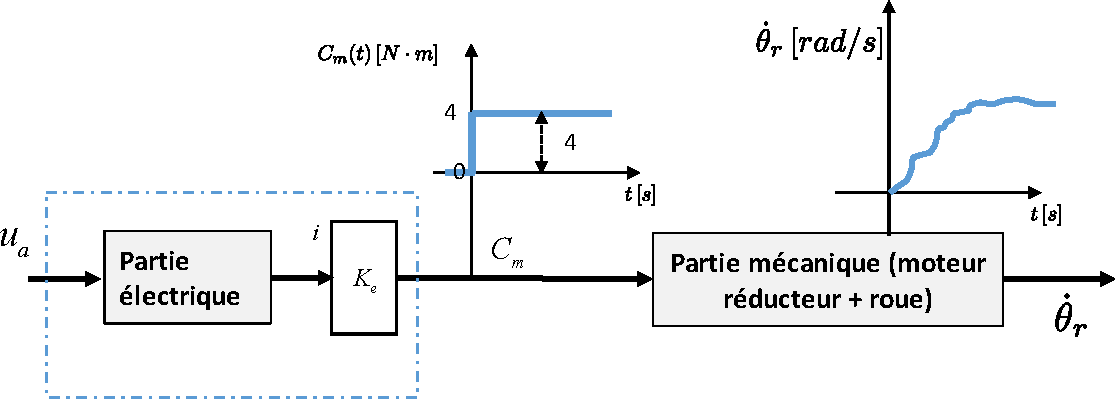
\includegraphics[width=1.0\textwidth]{essai_exp.pdf}
\caption{Essai expérimental pour l'identification de la fonction de transfert de la partie mécanique  \label{essai_exp}}
\end{center}
\end{figure}

\begin{figure}[!htb]
\begin{center}
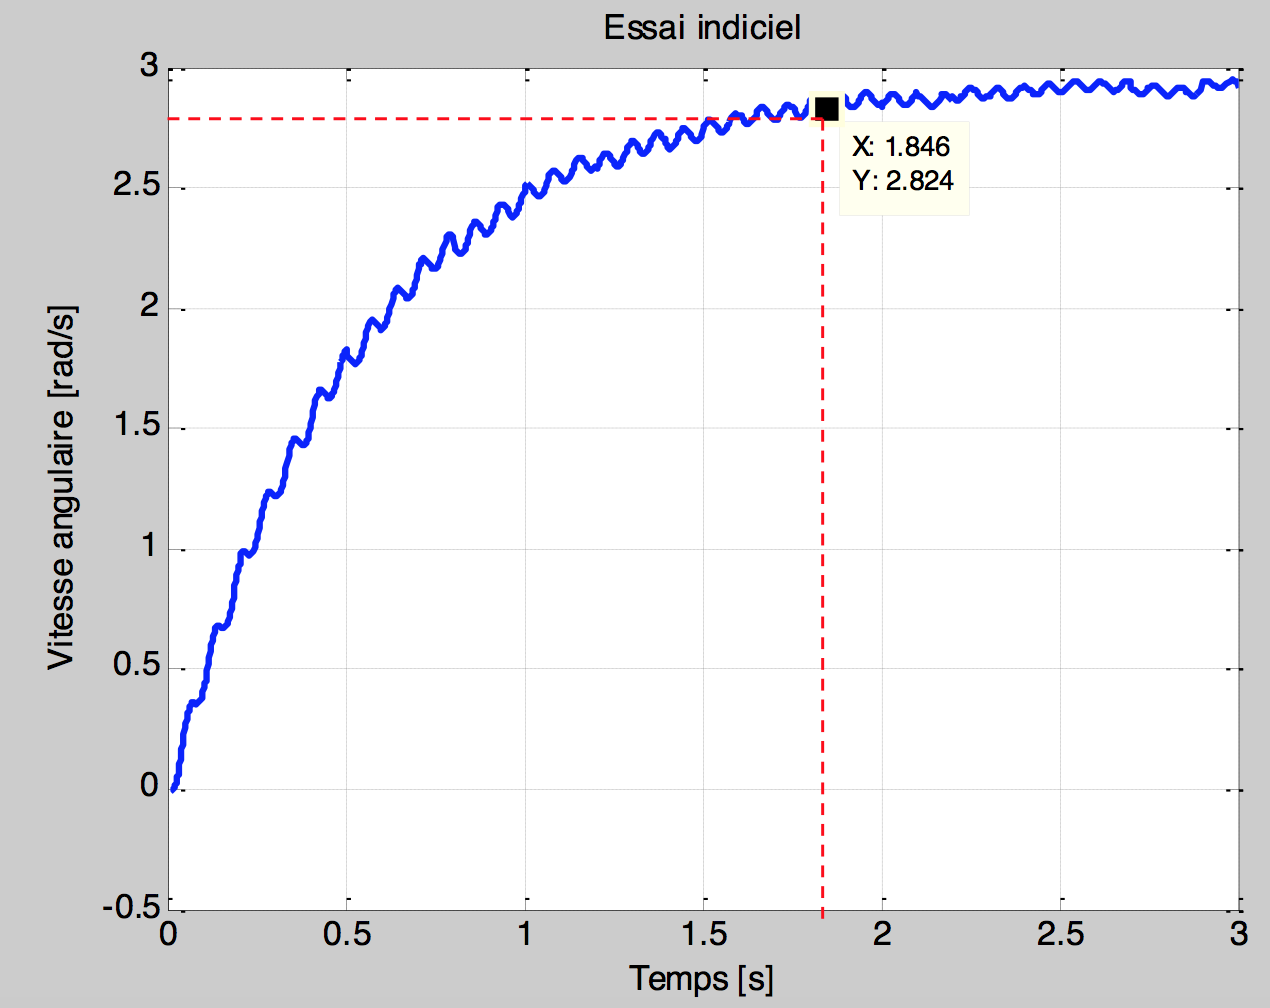
\includegraphics[width=0.6\textwidth]{reponse_echelon}
\caption{Réponse indicielle de la vitesse angulaire de la roue suite à un couple moteur d'un échelon 4 N.m  \label{reponse_echelon}}
\end{center}
\end{figure}